% ============= setup ============= %
% ======== package ======== %
\documentclass[mathserif]{beamer}
\usepackage{xeCJK}
\usepackage{graphicx}
\usepackage{xcolor}
\usepackage{setspace}
\usepackage{newtxmath}
\usepackage{ulem}

% ======== font ======== %
\setCJKmainfont{Taipei Sans TC Beta}
\setCJKsansfont{Taipei Sans TC Beta}
\AtBeginDocument{%
    \DeclareSymbolFont{pureletters}{OML}{cmm}{m}{it}%
    \SetSymbolFont{pureletters}{bold}{OML}{cmm}{b}{it}%
}
\hypersetup{
    colorlinks=true,
    linkcolor=black,
    urlcolor=blue
}

% ======== theme ======== %
\renewcommand{\baselinestretch}{1.25}
\usetheme{Madrid}
\usecolortheme{crane}
\setbeamertemplate{items}[circle]
\setbeamertemplate{section in toc}{\inserttocsectionnumber.~\inserttocsection}
\AtBeginSection[]{
    \begin{frame}
        \vfill
        \centering
        \begin{beamercolorbox}[sep=8pt,center,shadow=true,rounded=true]{title}
            \usebeamerfont{title}\insertsectionhead\par%
        \end{beamercolorbox}
        \vfill
    \end{frame}
}

% ======== data ======== %
\title{Windows 基本指令}
\author{temmie}
\date{}

% ============= setup ============= %

\begin{document}

\begin{frame}
    \titlepage
\end{frame}

\begin{frame}
    \tableofcontents
\end{frame}

\section{指令簡介}

\begin{frame}
    \frametitle{為什麼要學打指令}
    \begin{itemize}
        \item \sout{因為很帥}
        \item<2-> 提高效率:可以快速在資料夾移動或是開啟應用程式
        \item<2-> 簡化操作:一些安裝包可以略過設定
    \end{itemize}
\end{frame}

\begin{frame}
    \frametitle{如何使用指令}
    \begin{enumerate}
        \item 打開開始選單,尋找「命令提示字元」\\
        (或是使用快捷鍵 windows+R,接著打「cmd」)
        \item<2-> 輸入指令
    \end{enumerate}
\end{frame}

\begin{frame}
    \frametitle{如何使用指令}
    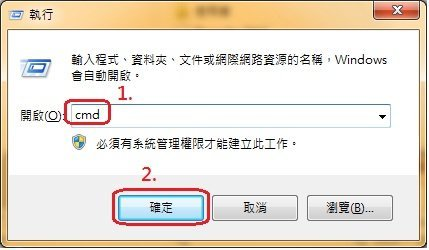
\includegraphics[width=8.0cm]{img/cmd_1.jpg}
\end{frame}

\begin{frame}
    \frametitle{如何使用指令}
    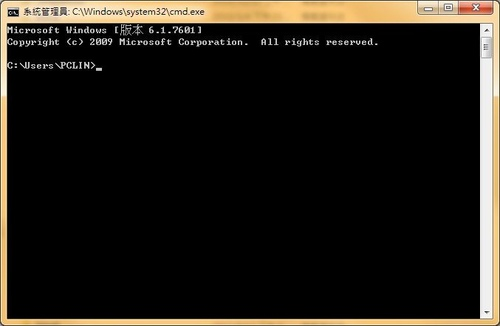
\includegraphics[width=8.0cm]{img/cmd_2.jpg}
\end{frame}

\section{目錄結構}

\begin{frame}
    \frametitle{目錄結構}
    \begin{itemize}
        \item 根目錄:Windows 系統下最上層的目錄,路徑為「\textcolor{red}{C:$\backslash$}」
        \item 系統目錄:Windows 系統中存放操作系統檔案的目錄,路徑為「\textcolor{red}{C:$\backslash$Windows}」
        \item 用戶目錄:用來個別儲存每個用戶自己的資料,路徑為「\textcolor{red}{C:$\backslash$User$\backslash$[name]}」
    \end{itemize}
\end{frame}

\begin{frame}
    \frametitle{目錄結構}
    \begin{itemize}
        \item 現在目錄:路徑為「\textcolor{red}{.}」
        \item 上一個目錄:路徑為「\textcolor{red}{..$\backslash$}」
        \item 上上一個目錄:路徑為「\textcolor{red}{..$\backslash$..$\backslash$}」
        \item 下一個目錄:路徑為「\textcolor{red}{[name]$\backslash$}」
        \vspace{0.5cm}
        \item 這個被稱作檔案的\textbf{「相對路徑」},如果要引入檔案就會用到!
    \end{itemize}
\end{frame}

\begin{frame}
    \frametitle{查看目錄結構}
    \begin{itemize}
        \item 你可以在 cmd 裡面使用指令「\textcolor{red}{tree}」,就可以查看當前目錄的樹狀結構
    \end{itemize}
\end{frame}

\section{常用指令}

\begin{frame}
    \frametitle{切換資料夾}
    \begin{itemize}
        \item CD:Change Directory(變更資料夾)
        \vspace{0.5cm}
        \item<2-> \textcolor{red}{CD [path]}:切換資料夾位置
        \item<2-> \textcolor{red}{CD$\backslash$}:返回到根目錄
        \item<2-> \textcolor{red}{CD..}:返回上一個目錄
    \end{itemize}
\end{frame}

\begin{frame}
    \frametitle{操作資料夾}
    \begin{itemize}
        \item MD:Make Directory(建立資料夾)
        \item RD:Remove Directory(刪除資料夾)
        \vspace{0.5cm}
        \item<2-> \textcolor{red}{MD [name]}:切換資料夾位置
        \item<2-> \textcolor{red}{RD [name] [/S] [/Q]}:刪除資料夾
        \begin{itemize}
            \item<2-> \textcolor{red}{/S}:刪除資料夾裡面的所有子目錄跟檔案
            \item<2-> \textcolor{red}{/Q}:不需要確認即可刪除
        \end{itemize}
    \end{itemize}
\end{frame}

\begin{frame}
    \frametitle{複製與刪除檔案}
    \begin{itemize}
        \item COPY:Copy(複製檔案)
        \item DEL:Delete(刪除檔案)
        \vspace{0.5cm}
        \item<2-> \textcolor{red}{COPY [/N] [source] [target]}:從 source 複製檔案到 target
        \begin{itemize}
            \item<2-> \textcolor{red}{/N}:如果目標已經有該檔案,則新的檔名複製
        \end{itemize}
        \item<2-> \textcolor{red}{DEL [/Q] [name]}:將檔案刪除
        \begin{itemize}
            \item<2-> \textcolor{red}{/Q}:不需要確認即可刪除
        \end{itemize}
    \end{itemize}
\end{frame}

\begin{frame}
    \frametitle{雜項}
    \begin{itemize}
        \item TAB 自動補全:在打指令或路徑時,可以按下 TAB 鍵,可以自動補全指令
        \item \textcolor{red}{CLS}:Clear Screen,將 cmd 清空
    \end{itemize}
\end{frame}

\begin{frame}
    \frametitle{總結}
    \begin{itemize}
        \item 指令通常不需要硬背用法,用多了自然會習慣
        \item 這種命令的使用會在 git 這個單元介紹更多東西
        \item 善用指令,讓你的工作方式更有效率!
    \end{itemize}
\end{frame}

\end{document}